\begin{frame}
    \begin{minipage}{0.45\textwidth}
        \textbf{\underline{Current Approach} - Fine Tuning:}

        \vspace{0.5em}
        
        \begin{itemize}
            \item Faster to train.
            \item More powerful networks.
            \item Uses network's pre-learned patterns.
        \end{itemize}

        \vspace{0.5em}

    \end{minipage}%
    \hfill
    \begin{minipage}{0.45\textwidth}
        \centering
        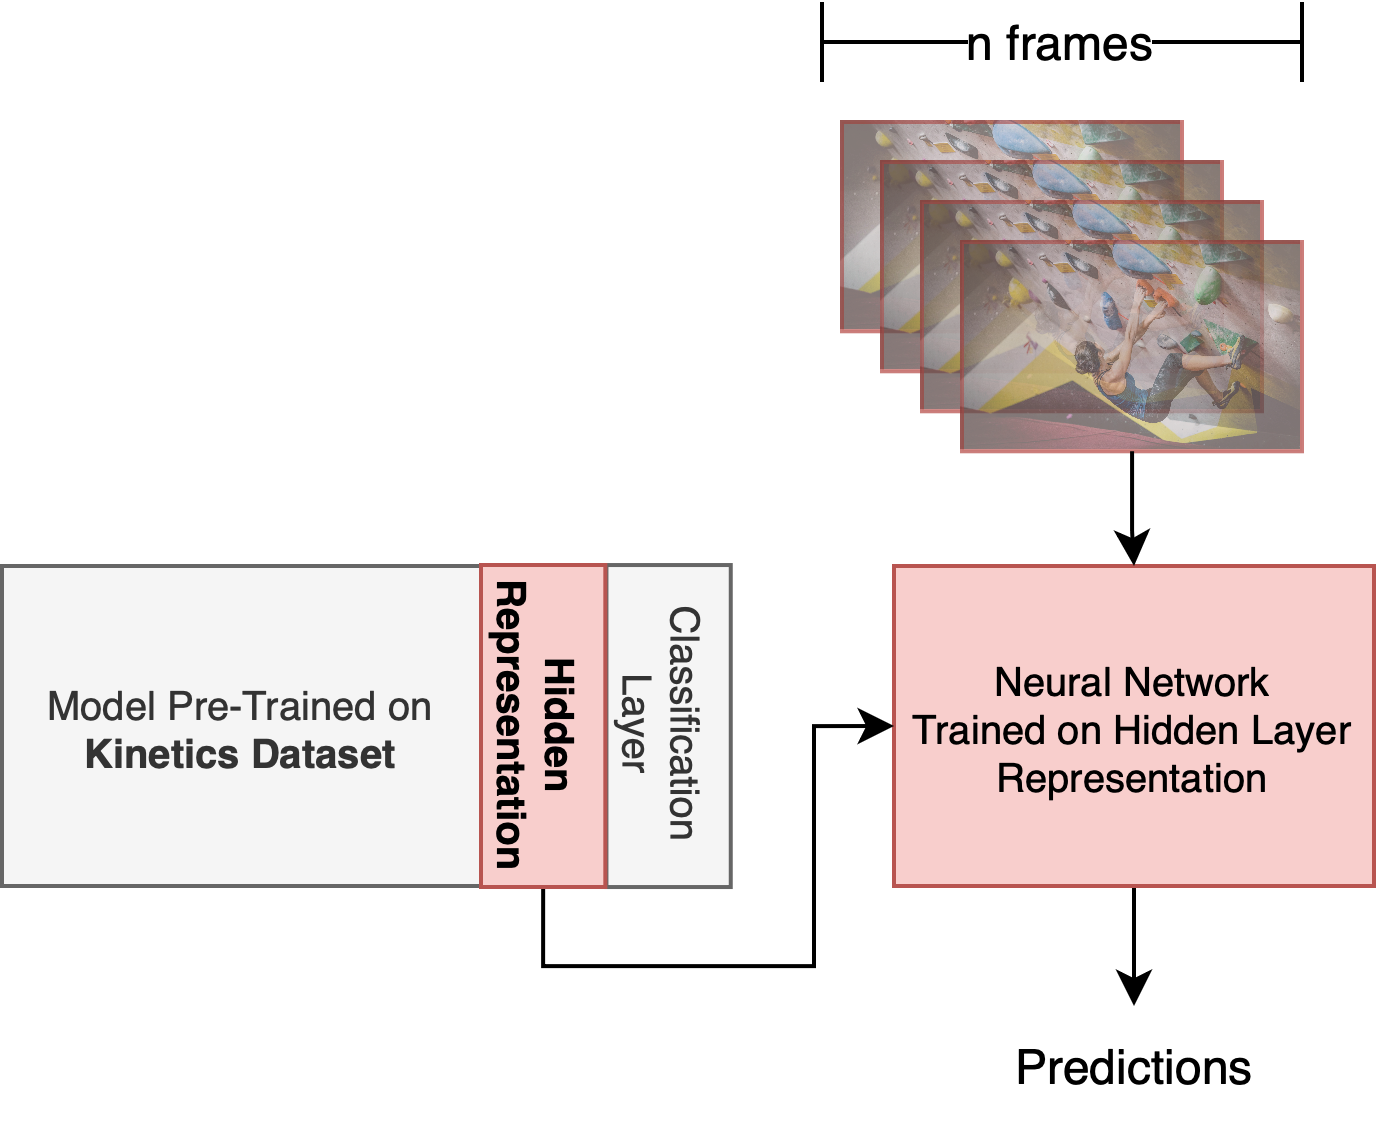
\includegraphics[width=\textwidth]{assets/visuals/fine-tuning-approach.drawio.png}

    \end{minipage}
\end{frame}

% NOTE: say that: "we basically remove the last layer of the network and use the previous layer as a feature extractors and we put a simple MLP on top of it for doing classifications on this layer."
% NOTE: explain quickly what is fine tuning.
% NOTE: remind that the kinetics dataset include sports related activities.

% NOTE: the networks trained on huge datasets such as the kinetics 690 contains a lot of activities.
% --- --- ---
% NOTE: justify and discuss the results we got, maybe imprecision, not enough fine tuning / training, etc.